\documentclass[german,oneside]{thesisclass}
% Based on thesisclass.cls of Timo Rohrberg, 2009
% ----------------------------------------------------------------
% Thesis - Main document
% ----------------------------------------------------------------


%% -------------------------------
%% |  Information for PDF file   |
%% -------------------------------
\hypersetup{
 pdfauthor={Wolfgang Heni, Sebastian Heunisch},
 pdftitle={Labor Nanotechnologie - OLED},
 pdfsubject={Herstellung Organischer Leuchtdioden},
 pdfkeywords={OLED}
}


%% ---------------------------------
%% | Information about the thesis  |
%% ---------------------------------

\newcommand{\myname}{Wolfgang Heni \\ Sebastian Heunisch}
\newcommand{\mytitle}{Organische Leuchtdioden}
\newcommand{\myinstitute}{Lichttechnischel Institut (LTI)}

\newcommand{\reviewerone}{?}
\newcommand{\reviewertwo}{?}
\newcommand{\advisor}{Dipl.-Ing Tobias Bocksrocker}
\newcommand{\advisortwo}{?}

\newcommand{\timestart}{XX. Monat 20XX}
\newcommand{\timeend}{XX. Monat 20XX}
\newcommand{\submissiontime}{DD. MM. 20XX}


%% ---------------------------------
%% | ToDo Marker - only for draft! |
%% ---------------------------------
% Remove this section for final version!
\setlength{\marginparwidth}{20mm}

\newcommand{\margtodo}
{\marginpar{\textbf{\textcolor{red}{ToDo}}}{}}

\newcommand{\todo}[1]
{{\textbf{\textcolor{red}{(\margtodo{}#1)}}}{}}


%% --------------------------------
%% | Old Marker - only for draft! |
%% --------------------------------
% Remove this section for final version!
\newenvironment{deprecated}
{\begin{color}{gray}}
{\end{color}}


%% --------------------------------
%% | Settings for word separation |
%% --------------------------------
% Help for separation:
% In german package the following hints are additionally available:
% "- = Additional separation
% "| = Suppress ligation and possible separation (e.g. Schaf"|fell)
% "~ = Hyphenation without separation (e.g. bergauf und "~ab)
% "= = Hyphenation with separation before and after
% "" = Separation without a hyphenation (e.g. und/""oder)

% Describe separation hints here:
\hyphenation{
% Pro-to-koll-in-stan-zen
% Ma-na-ge-ment  Netz-werk-ele-men-ten
% Netz-werk Netz-werk-re-ser-vie-rung
% Netz-werk-adap-ter Fein-ju-stier-ung
% Da-ten-strom-spe-zi-fi-ka-tion Pa-ket-rumpf
% Kon-troll-in-stanz
}


%% ------------------------
%% |    Including files   |
%% ------------------------
% Only files listed here will be included!
% Userful command for partially translating the document (for bug-fixing e.g.)
\includeonly{%
titlepage,
introduction,
content,
appendix
}


%%%%%%%%%%%%%%%%%%%%%%%%%%%%%%%%%
%% Here, main documents begins %%
%%%%%%%%%%%%%%%%%%%%%%%%%%%%%%%%%
\begin{document}

% Remove the following line for German text
%\selectlanguage{english}

\frontmatter
\pagenumbering{roman}
%% titlepage.tex
%%

% coordinates for the bg shape on the titlepage
\newcommand{\diameter}{20}
\newcommand{\xone}{-15}
\newcommand{\xtwo}{160}
\newcommand{\yone}{15}
\newcommand{\ytwo}{-253}

\begin{titlepage}
% bg shape
\begin{tikzpicture}[overlay]
\draw[color=gray]  
 		 (\xone mm, \yone mm)
  -- (\xtwo mm, \yone mm)
 arc (90:0:\diameter pt) 
  -- (\xtwo mm + \diameter pt , \ytwo mm)
	-- (\xone mm + \diameter pt , \ytwo mm)
 arc (270:180:\diameter pt)
	-- (\xone mm, \yone mm);
\end{tikzpicture}
	\begin{textblock}{10}[0,0](4,2.5)
		
\includegraphics[width=.3\textwidth]{logos/KITLogo_RGB.pdf}
	\end{textblock}
	\changefont{phv}{m}{n}	% helvetica	
	\vspace*{2cm}
	\begin{center}
		\huge{\mytitle}
		\vspace*{2cm}\\
		\Large{
			\iflanguage{english}{Diploma Thesis of}			
												  {Laborbericht\\von}
		}\\
		\vspace*{1cm}
		\huge{\myname}\\
		\vspace*{1cm}
		\Large{
			\iflanguage{english}{At the faculty of Computer Science}			
													{An der Fakult\"at Elektro- und Informationstechnik}
			\\
			\myinstitute
		}
	\end{center}
	\vspace*{1cm}
\Large{
\begin{center}
\begin{tabular}[ht]{l c l}
%  \iflanguage{english}{Reviewer}{Erstgutachter}: & \hfill  & \reviewerone\\
%  \iflanguage{english}{Second reviewer}{Zweitgutachter}: & \hfill  & \reviewertwo\\
  \iflanguage{english}{Advisor}{Betreuer}: & \hfill  & \advisor\\
%  \iflanguage{english}{Second advisor}{Zweiter betreuender Mitarbeiter}: & \hfill  & \advisortwo\\
\end{tabular}
\end{center}
}


\vspace{2cm}
%\begin{center}
%\large{\iflanguage{english}{Time (?)}{Bearbeitungszeit}: \timestart \hspace*{0.25cm} -- \hspace*{0.25cm} \timeend}
%\end{center}


\begin{textblock}{10}[0,0](4,16.8)
\tiny{ 
	\iflanguage{english}
		{KIT -- University of the State of Baden-Wuerttemberg and National Laboratory of the Helmholtz Association}
		{KIT -- Universit�t des Landes Baden-W�rttemberg und nationales Forschungszentrum der Helmholtz-Gesellschaft}
}
\end{textblock}

\begin{textblock}{10}[0,0](14,16.75)
\large{
	\textbf{www.kit.edu} 
}
\end{textblock}

\end{titlepage}

\blankpage


%% -------------------
%% |   Directories   |
%% -------------------
\tableofcontents
\blankpage


%% -----------------
%% |   Main part   |
%% -----------------
\mainmatter
\pagenumbering{arabic}
%% introduction.tex
%%

%% ==============================
\chapter{Einleitung}
\label{ch:Introduction}
%% ==============================
Organische Leuchtdioden (engl. \textit{organic light emitting diode} - OLED) werden heute bereits in zahlreichen Ger�ten verwendet. Seit Anfang der 90er Jahre haben sie sich rasch entwickelt. Man kann mit ihnen inzwischen optoelektronische Anzeige mit gro�em Farbraum und hoher Aufl�sung herstellen. So findet man zahlreiche Smartphones auf dem Markt die OLEDs als Displaytechnologie verwenden.

Auch als Leuchtmittel sind OLEDs eine vielversprechende Technologie. Im Gegensatz zu anorganischen LEDs sind OLEDs keine Punktlichtquelle, sondern Fl�chenstrahler. Dies er�ffnet vielf�ltige neue Gestaltungsm�glichkeiten in der Allgemeinbeleuchtung. Da OLEDs eine Lichtausbeute besitzen, die mit anorganischen LEDs vergleichbar ist, lassen sich in der Beleuchtungstechnik Energie und damit auch Kosten sparen.

Die Herausforderung bei der Herstellung von OLEDs besteht darin, die Lebensdauer zu verl�ngern, die Herstellungskosten weiter zu senken und die Lichtausbeute zu steigern. Daher sind OLEDs auch am LTI Gegenstand intensiver Forschung. Darum wird auch im Labor Nanotechnologie ein Versuch durchgef�hrt, indem eine Einf�hrung in die Herstellung von OLEDs gegeben wird.
% 
% Nach intensiver Forschung sind die Preise f�r die Herstellung von OLEDs sind in den letzten Jahren stark gefallen. Hieran wird weiter intensiv geforscht.
% 
% Auch als Leuchtmittel ist sind OLEDs eine vielversprechende Technologie. So lassen sich mit ihnen effiziente Fl�chenstrahler herstellen.


%% content.tex
%%

%% ==============
\chapter{Grundlagen}
\label{ch:Grundlagen}
%% ==============
\section{Ladungstr�gerinjektion}
\label{ch:Grundlagen:sec:Injektion}

\section{PEDOT:PSS}
\label{ch:Grundlagen:sec:PEDOT}

\section{Lichterzeugung}
\label{ch:Grundlagen:sec:Lichterzeugung}




%% ===========================
\section{OLED}
\label{ch:Grundlagen:sec:OLED}
%% ===========================
\chapter{Versuchsdurchf�hrung}
\section{Herstellung}
\label{ch:Herstellung}
Als Ausgangsmaterial f�r die im Praktikum hergestellten OLEDs wurde Glas\-substrat verwendet, dass mit einer 120 nm dicken Schicht Indiumzinnoxid (englisch \textit{indium tin oxide} - ITO) beschichtet ist. Aus diesem Substrat wurden mit dem Glasschneider zun�chst 8 16~x~16~mm$^2$ gro�e Proben geschnitten. Nun wurde 3/4 der Probenfl�che mit einem Klebestreifen abgeklebt und anschlei�end 7~min in ein Bad aus 37~\%iger Salzs�ure gegeben, das mit einer Spartelspitze Zinkpulver versetzt wurde. Hierdurch wird das ITO im nicht abgeklebten Bereich wegge�tzt. Dieser Bereich dient sp�ter zur Kontaktierung der Metallfl�chen. Nach dem �tzprozess wurden die Proben mit Wasser abgesp�hlt und der Klebestreifen abgezogen. Die beschriebene Vorbereitung der Proben wurde im Vorfeld des Versuchs durch Tobias Bocksrocker durchgef�hrt.

Die Proben wurden nun in einem Becherglas Aceton 10~min in ein Ultraschallbad gestellt. Danach werden die Proben aus dem Aceton genommen und in Isopropanol weitere weitere 10~min mit Ultraschall gereinigt. Durch die Reinigung mit Aceton werden Fette und Schmutz von der Oberfl�che der Proben gel�st. Im Isopropanol l�sen sich weitere R�ckst�nde, die sich in Aceton nicht l�sen. Au�erdem werden durch das Isopropanol auch Acetonreste gel�st. Nach der Reinigung durch Isopropanol wurden die Proben mit Stickstoff trockengeblasen und anschlie�end f�r 2~min in einen Plasmaverascher gelegt. Hierin sind die Proben einem Sauerstoffplasma ausgesetzt. Die darin enthaltenen Sauerstoffradikale f�hren zum einen dazu, dass organische Reste auf der Oberfl�che verbrennen. Zum anderen lagern sich auch Sauerstoffatome an der Oberfl�che des ITO an. Diese sogenannte Aktivierung f�hrt dazu, dass die Oberfl�che polar wird, und sich somit Polare L�sungen auf der Oberfl�che besser verteilen. Au�erdem wird auch die Austrittsarbeit des ITO erh�ht. Nach dem Plasmaveraschen wurden die Proben mit einem Wasserfesten Folienstift auf der Glasseite durchnummeriert, damit sie im Folgenden unterscheidbar sind.

Als n�chstes wurde eine PEDOT:PSS-Wasser-L�sung im Verh�lltnis 1:1 hergestellt.\todo{evtl PSS erw�hnen}  Hierzu wurden zun�chst 750~$\upmu$l PEDOT:PSS mit einem Membranfilter gefiltert und anschlie�end 750~$\upmu$l Reinstwasser hinzugegeben. Um die L�sung zu durchmischen und Polymerklumpen zu vermeiden, wird die L�sung in ein Ultraschallbad mit niedriger Leistung (110~W) gegeben. Die Polymerl�sung "`Super Yellow"' wurde bereits einen Tag vorher von Tobias Bocksrocker hergestellt, da diese mindestens 24~h zum durchmischen ben�tigt.

Die Proben wurden nun zusammen mit der PEDOT:PSS-L�sung in eine Glove-Box mit Stickstoffatmosph�re geschleust. Hierzu wurde die Schleusenkammer drei mal evakuiert und mit Stickstoff geflutet um zu vermeiden, dass Sauerstoff mit in die Glove-Box geschleust wird. Die Stickstoffatmosph�re ist notwendig, da das Polymer "`Superyellow"' Sauerstoffempfindlich ist. Nun wurde per Spin-Coating eine Schicht aus PEDOT:PSS aufgebracht. Hierzu wurden mit einer \todo{Eppendorf-Pipette??}\todo{Luftpolsterpipette} 150~$\upmu$l PEDOT:PSS-L�sung gleichm��ig auf dem Substrat verteilt. Das Substrat wurde durch eine Vakuumpumpe auf dem Drehteller des Spin-Coaters gehalten. Um die PEDOT:PSS-L�sung weiter auf dem Substrat zu verteilen wurde die Probe f�r 5 Sekunden mit 500 Umdrehungen pro Minuten im Spin-Coater \todo{gedreht}. Um die gew�nschte Schichtdicke der L�sung von $\sim18$~nm zu erhalten, wurde die Probe anschlie�end f�r 100 Sekunden mit 4000 Umdrehungen pro Minuten \todo{gedreht}. Durch die schnelle Drehung der Probe wurde die �berfl�ssige L�sung durch die Zentrifugalkraft zur Seite von der Probe geschleudert. Die Proben 1 und 2 wurden nicht mit PEDOT:PSS beschichtet.

Um das L�sungsmittel Wasser aus den PEDOT:PSS-Filmen zu Treiben wurden die Proben f�r 5 Minuten bei 130 �C im Vakuumofen gebacken. L�ngeres Backen w�rde zu einer h�heren Lebensdauer der hergestellten OLEDs f�hren, was f�r den durchgef�hrten Versuch aber nicht notwendig war.
Nach dem Backen wurden die Proben auf eine Metalloberfl�che zum Abk�hlen gelegt. \todo{Abk�hlen, da SuperYellwo sonst antrocknet}
Anschlie�end erfolgte das Auftragen der organischen Emitterschicht. Hierzu wurden 120~$\upmu$l "`Super Yellow"' pro Probe gleichm��ig auf dem Substrat verteilt. Um ein Antrocknen des "`Super Yellows"' musste der Spin-Coating Vorgang m�glichst schnell nach dem Aufbringen der L�sung gestartet werden. Tabelle \ref{tab:spin} zeigt die f�r die Proben 1 - 8 verwendete Einstellungen beim Aufschleudern des "`SuperYellows"'. 
 
\begin{table}%
\centering
\begin{tabular}{lcccccccc}
\toprule
Probennummer 																				& 1		&	2		&	3		&	4		&	5		&	6		&	7		&	8\\
 \midrule
$n_{\mathrm{Vorlauf}}$ / $\frac{1}{\mathrm{min}}$					&500	&500	&500	&	-		&500	&500	&500			&-\\ 
$t_{\mathrm{Vorlauf}}$ / s																&5		&5		&5		&		-	&5		&5		&5		&-\\																
$n_{\mathrm{Aufschleudern}}$ / $\frac{1}{\mathrm{min}}$		&1000	&1000	&	1000&500	&4000	&4000	&1000	&500\\
$t_{\mathrm{Aufschleudern}}$ / s													&55		&55		&55		&55		&55		&55		&55		&55\\			
\bottomrule 
\end{tabular}
\caption{Verwendete Spin-Coater Einstellungen beim Auftragen von "`Super Yellow"'}
\label{tab:spin}
\end{table}


Nach dem Aufbringen von "`Super Yellow"' wurden die Proben in einer gasdichten Transportbox aus der zum Spin-Coaten verwendeten Glove-Box zu einer weiteren Glove-Box transportiert, in der eine Anlage zur Verdampfung von Materialien ist. Zusammen mit einer Maske zur Definition der aufzudampfenden Kathoden wurde die Transportbox wie zuvor beschrieben in die Glove-Box geschleu�t.

Die Proben wurden mit Klebeband im Maskenhalter fixiert, und die Maske zur Definition der aufzudampfenden Strukturen dar�ber positioniert. Dies wurde von Tobias Bocksrocker durchgef�hrt. Daraufhin wurde die Maske mit den Proben in den Rezipienten des Verdampfungsanlage eingebaut, und dieser �ber ein Vakuumpumpsystem auf einen Basisdruck von $p_{\mathrm{basis}}~\approx~6~\cdot~10^{-7}~$mbar abgepumpt.

Bei geschlossener Blende, die die Proben vor dem Aufdampfen von Material sch�tzt, wurde der in der Verdampfungsanlage verbaute Wolframtiegel mit Calcium (Ca) langsam erhitzt. Hierzu wurde der Heizstrom langsam erh�ht. Bei einer zu schnellen Erhitzung des Tiegels droht eine Verpuffung des Ca.
Die Aufdampfrate in der Anlage wurde durch einen Schwingquarz gemessen, der zuvor auf das verwendete Material kalibriert werden musste. Hierzu wurde die Dichte $\rho_{\mathrm{Ca}}~=~1.55~$g/cm$^3$ eingestellt. Bei einem Strom von $\sim$165~A wurde eine Aufdampfrate von $\sim$1,5$~\mathring{\mathrm{A}}$/s gemessen. Bei rotierendem Probenhalter wurde die Blende ge�ffnet und ein Ca-Film mit einer Schichtdicke von $d_{\mathrm{Ca}}~=~50~\mathring{\mathrm{A}}$ aufgedampft. Danach wurde die Blende geschlossen. Die Rotation des Probenhalters diente zum Ausgleich von inhomogenem Aufdampfen. 
Anschlie�end wurde der Tiegel langsam durch Verringerung des Heizstromes abgek�hlt. 

Daraufhin wurde ein mit Aluminium (Al) gef�llter Tiegel langsam erhitzt. Hier wurde zur Messung der Aufdampfrate eine Dichte von $\rho_{\mathrm{Al}}~=~2,7~$g/cm$^3$ eingestellt. Bei einem Heizstrom von $\sim260$~A wurde eine Aufdampfrate von $\sim3~\mathring{\mathrm{A}}$/s gemessen. Nach dem �ffnen der Blende wurde unter Rotation des Probenhalters eine Al-Schicht mit einer Schichtdicke von $d_{\mathrm{Al}}~=~200~$nm aufgedampft. Daraufhin wurde die Blende geschlossen und das restliche Al aus dem Tiegel verdampft.

Nach dem Fluten des Rezipienten mit Stickstoff wurde der Probenhalter aus der Anlage ausgebaut und die Proben in die gasdichte Transportbox gelegt. Die Proben wurden in eine Glove-Box zur Messung und Charakterisierung der hergestellten OLEDs geschleu�t. Der zum Aufdampfen verwendete Probenhalter und die Maske wurden mit Isopropanol gereinigt. Die Hergestellten Proben sind nun f�r die Charakterisierung bereit.

Abbildung \ref{fig:OLED_Schema} zeigt den schematischen Aufbau der hergestellten OLEDs. Abbildung \ref{fig:OLEDOben} zeigt die Ansicht von oben. Zu erkennen sind die zwei zuvor aufgedampften Kathoden aus Ca und Al. Au�erdem ist im unteren Bereich der Probe ein heller Streifen zu erkennen. Hier wurde das ITO bei der Herstellung wegge�tzt. Beim Betrachten von Abbildung \ref{fig:OLEDSeite} ist der Aufbau der OLED von der Seite und der Schichtaufbau dieser zu erkennen. Der bei Anregung leuchtende Bereich ist durch die Fl�che bestimmt, der zwischen Anode (ITO) und Kathode (Al/Cu) liegt. Damit sind bei einer gro�en Anodenfl�che und den zwei aufgedampften Kathodenfl�chen zwei OLEDs pro Probe vorhanden. 

\begin{figure}%
\centering
\begin{adjustwidth}{0cm}{0cm}
	\subfloat[Ansicht von oben]{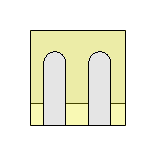
\includegraphics[width=.5\columnwidth]{Grafiken/OLED-Ansicht-Oben.pdf}\label{fig:OLEDOben}}
	\subfloat[Ansicht von der Seite]{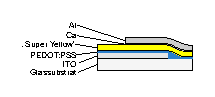
\includegraphics[width=.5\columnwidth]{Grafiken/OLED-Ansicht-Seite.pdf} \label{fig:OLEDSeite}}%
	\end{adjustwidth}
\caption[Schema: Hergestellte OLED]{Schematische Darstellung der hergestellten Proben. \textbf{(a)} Die Ansicht von oben zeigt die zwei Kathodenfl�chen (grau) sowie das organische Material (gelb). Im unteren bereich ist das Fehlen der ITO-Schicht zu erkennen. \textbf{(b)} Die Ansicht von der Seite zeigt den Schichtaufbau der hergestellten OLEDs. }%
\label{fig:OLED_Schema}%
\end{figure}



\section{Durchf�hrung der Messungen}
\label{ch:Messsystem}

Die Charakterisierung der OLEDs wurde, ebenfalls in Stickstoffatmosph�re, in einem "`OLED Characterisation System"' (OCS) durchgef�hrt. Die Proben wurden zun�chst in einen Rahmen gelegt, der in eine Halterung des OCS gesteckt wurde. Zur Kontaktierung der OLEDs werden nun Kontaktstifte an die Proben gedr�ckt. Die Steuerung des OCS und die Aufnahme der Messdaten erfolgt durch das Programm "`Kennlinie.exe"'.  Durch das Anlegen einer Spannung von 3~V wurden die OLEDs nun auf Funktionsf�higkeit �berpr�ft. Die augenscheinlich Bessere der Beiden wurde im Folgenden analysiert.

Zun�chst wurde die zu untersuchende OLED mit Hilfe eines Lasers mittig ausgerichtet. Nach dem schlie�en der Abdeckung am OCS wurde nun die Automatisierte Messung gestartet. Bei der Messung wird die OLED aus der Ladeposition zu einem Spektrometer hin gedreht. 

Die Aufzeichnung der Messdaten erfolgte an einem Computer mit dem Programm "`\textit{kennlinie.exe}"'. Zur Messung wurde ein Spannungsbereich von 0 - 10~V eingestellt, der in 0,5~V Schritten durchlaufen wurde. F�r die Spektroskopie wurde ein Wellenl�ngenbereich von 300 - 800~nm gew�hlt, die in Schritten von 1~nm durchlaufen wurden. Die Integrationszeit des Sensors betrug 10~ms. 


\chapter{Auswertung der Messergebnisse}
\label{ch:Messung}

\section{Fehlerhafte Messungen}
\label{ch:Messung:sec:Fehler}
Bei der Durchf�hrung der Messungen traten verschiedene Effekte auf, die so nicht zu erwarten waren und auf einen Fehler im Messsystem hindeuten. 

Bei der Aufzeichnung der Spektren der Proben zeigte sich, dass sich die Maxima der Bestrahlungsst�rke unterschiedlicher Spannungen stark ver�nderte. In Abbildung \ref{fig:Verschiebung} ist die deutliche Abweichung von den Messungen bei den Spannungen $U$~=~9~V (braun) und $U$~=~8~V (hellblau?) \todo{die 3 blaut�ne sin etwas ungeschickt} zu erkennen. Auch bei $U$~=~5~V (gr�n) zeigt sich eine Abweichung zu den Maxima der anderen Spannungen.

Dieses Verhalten ist bei Messungen aller Proben zu beobachten. Die Spannungen bei denen die Abweichungen der Maxima auftreten, sind zuf�llig verteilt.

Da das Emissionsspektrum der hergestellten Proben Materialabh�ngig ist und von der Energiedifferenz zwischen HOMO und LUMO abh�ngt ist eine solche �nderung des Spektrums physikalisch nicht sinnvoll.  Es wird daher angenommen, dass diese Messungen fehlerhaft sind.
\begin{figure}%
\centering
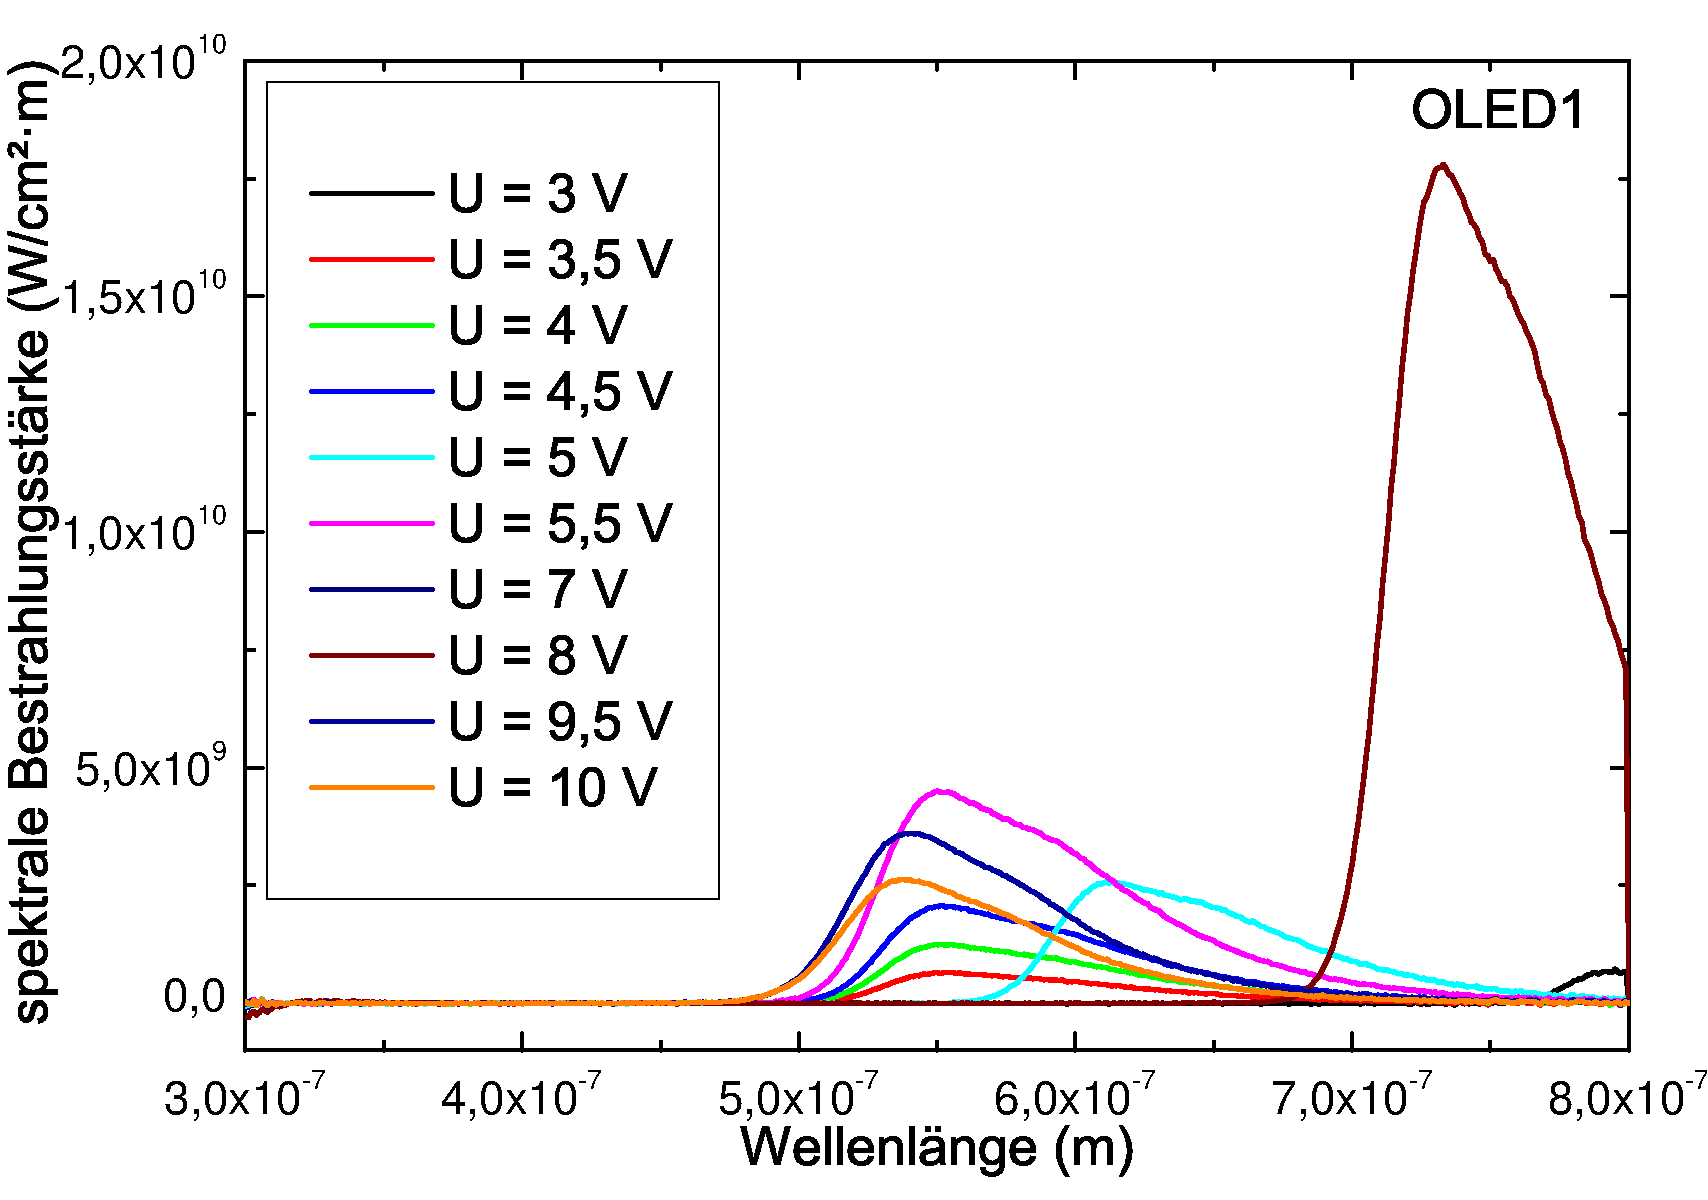
\includegraphics[width=.6\columnwidth]{Grafiken/Verschiebung.pdf}%
\caption[OLED1: Bestrahlungsst�rkespektrum]{Die Abbildung zeigt die Bestrahlungsst�rke  der Probe OLED1 in Abh�ngigkeit von der Wellenl�nge. F�r unterschiedliche OLED-Betriebsspannungen liegen die Maxima der Bestrahlungsst�rke bei unterschiedlichen Wellenl�ngen. Spannungswerte bei denen es zur Aussteuerung des Messsystems kam sind ausgeblendet.
}%
\label{fig:Verschiebung}%
\end{figure}

%
%Verschiebeung der Spektren
%	Unterschiedliche Spannungen - unterschiedliche Proben
%	
%
%Fehlen einzelner Spektren bei bestimmten Spannungswerten
%	Kontaktprobleme?
%	
%
%---> entsprechender Spannungswert nicht auswertbar

Beim Betrachten der Bestrahlungsst�rke der hergestellten Proben zeigt sich ein Aussteuern des Messsystems. Eine Verringerung der Integrationszeit von 30~ms auf 10~ms erm�glichte eine Aussteuerfreie Messung bis zu einer Spannung von $U~\approx~5~$V. Bei h�heren Spannungen war die Bestrahlung durch die hergestellten OLEDs zu hoch. Abbildung \ref{fig:Aussteuern} zeigt das Aussteuern ab einer Spannung von 5,5~V (rosa).

Aufgrund der aufgetretene Messfehler ist eine Auswerung der Messdaten nur eingeschr�nkt m�glich. Eine Auswertung der aus dem Spektrum abgeleiteten Gr��en, bei Spannungen, die die beschriebenen Fehler aufweisen, ist nicht sinnvoll. 


\begin{figure}%
\centering
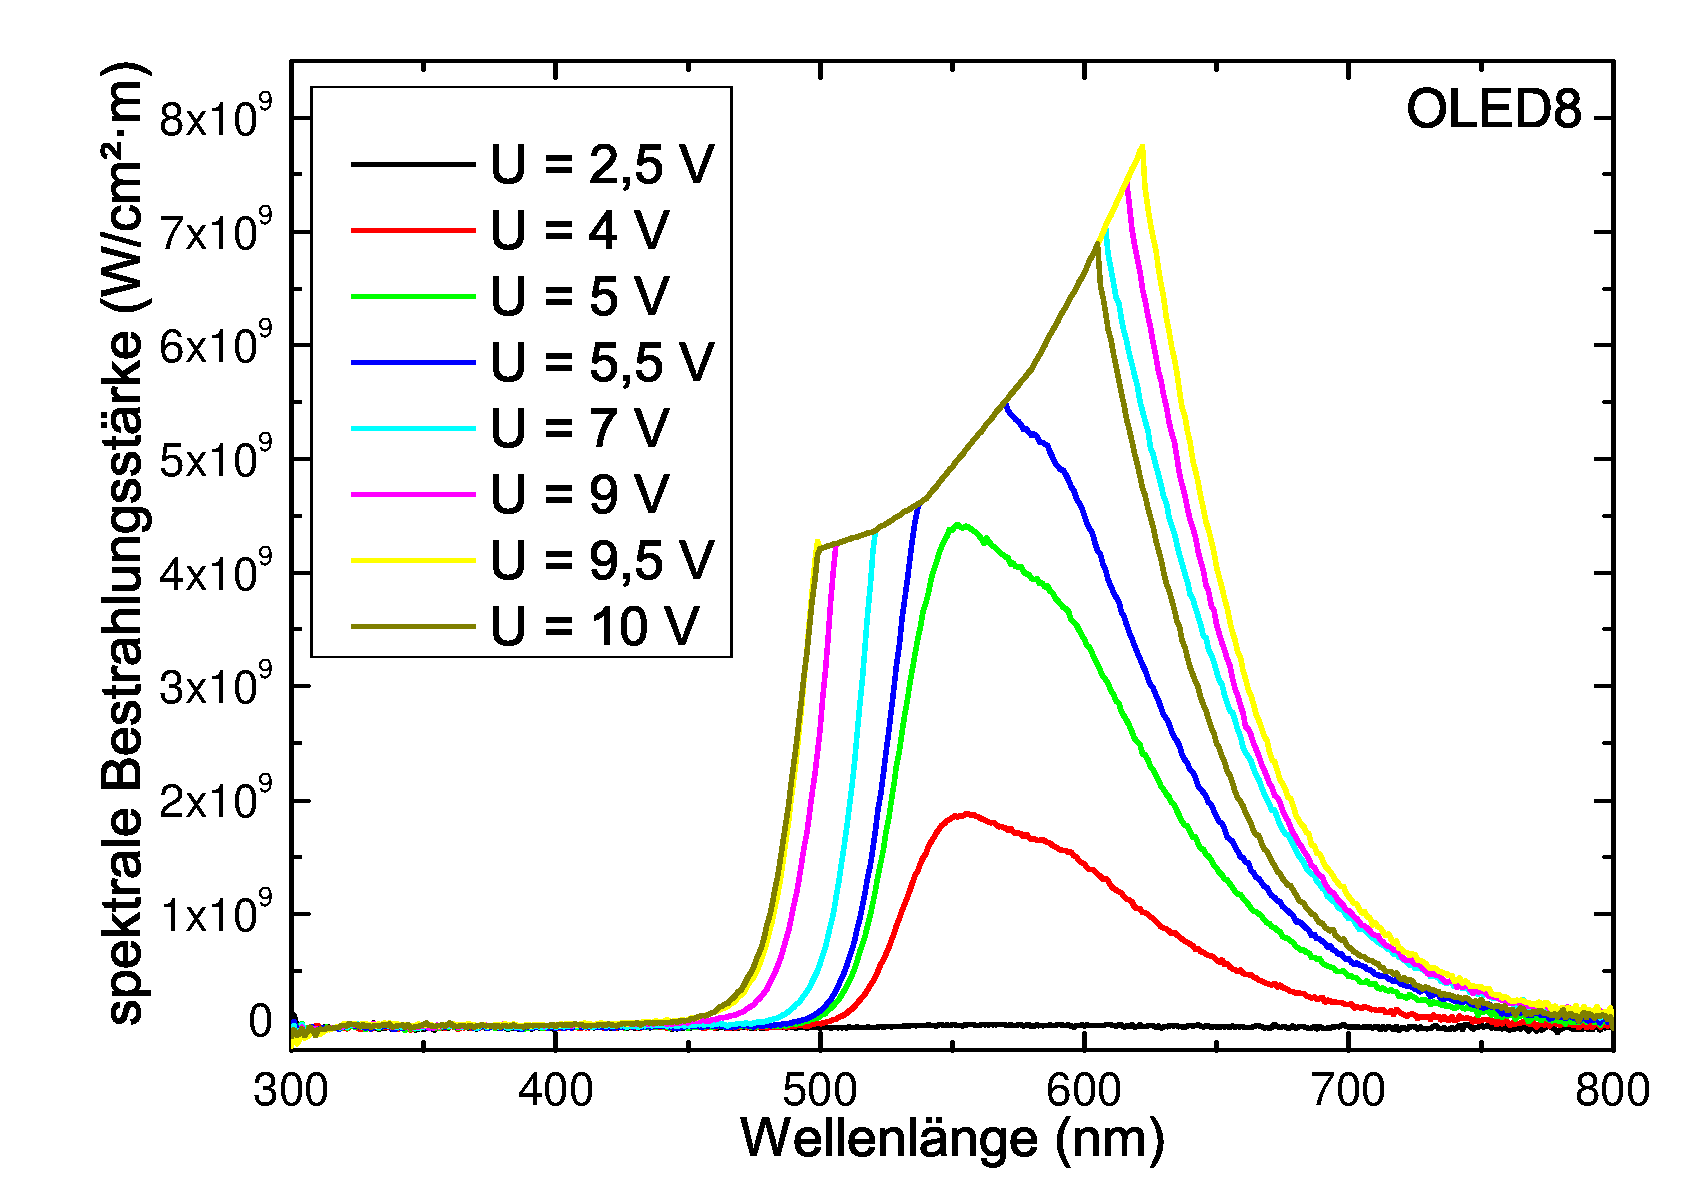
\includegraphics[width=.6\columnwidth]{Grafiken/Aussteuern.pdf}%
\caption[OLED8: Aussteuerung des Messsystems]{Die Abbildung zeigt die Bestrahlungsst�rke der Probe OLED8 in Abh�ngigkeit von der Wellenl�nge bei OLED-Betriebsspannungen von 4~V bis 6,5~V. Ein Aussteuern des Messsystems ist ab einer Spannung von 5,5~V erkennbar.}%
\label{fig:Aussteuern}%
\end{figure}

%Aussteuerung des Sensor bei ~5 V
%	- reduzierung von tintegration von 30 auf 10 ms
%	- wartezeit zw. 2 messungen: 1 s 
%	hat nix gebracht
%
%-> Werte oberhalt 5 V nicht verwertbar
%
%
%Evtl. 4 und 7 verschrtauscht
%
%
%OLED6 ist schei�e!
%	a.) Nicht die d�nnste, sondern die Dickste, weil zu lange gewartet vor Spin-Coating: -> Angedrocknet: eher unwarscheinlich
%	
%	b.) Probleme mit der Kontaktierung -> dadurch viel h�herer Wdstd. bzw. garkeine messung!
%	
	


\section{Stromdichte/Spannung-Kennlinien}
\label{ch:Messung:sec:jU}
%Anhand von Stromdichte/Spannungs ($j/U$)-Kennlinen l�sst sich die Stromdichte in Abh�ngigkeit der angelegten Spannung �ber die OLED
OLEDs zeigen beim betrachten der Stromdichte/Spannung ($j/U$)-Kennline �hnlichkeit zu einer Diodenkennlinie. Abbildung \ref{fig:jUPEDOT} zeigt dieses Verhalten Anhand einiger Messungen. Bis zu einer Spannung von 2,5~V ist kein Stromfluss zu beobachten. Die Verschiebung der Potentiale durch die angelegte Spannung reicht noch nicht aus um Ladungstr�ger zu injizieren (vgl. \ref{ch:Grundlagen:sec:Injektion}). 

Ab der Grenzspannung U$_\mathrm{G}~\approx~$3~V ist bei Erh�hung der Spannung ein exponentieller Anstieg der Stromdichte zu beobachten. Ab U$_\mathrm{G}~\approx~$8~V flachen die Kurven ab. Die Begrenzung des Stroms ist zum einen durch die Besetzung der Zust�nde an der Grenzfl�che zu den Elektroden zu erkl�ren \todo{ref}. Zum anderen ist auf Grund der geringen Beweglichkeit eine hohe Ladungstr�gerdichte erforderlich um hohe Stromdichten zu erreichen. Die hohe Ladungstr�gerdichte erzeugt jedoch eine Raumladungszone die den Stromfluss begrenzt \cite{SCD}.   
Bei einer weiteren erh�hung der Spannung w�re eine Zerst�rung der OLEDs zu erwarten. Bei hohen Stromdichten droht eine �berhitzung der organischen Schicht, was zu einer Degradation dieser f�hrt und die Lebensdauer der Leuchtdiode stark verk�rzt. 

\begin{figure}%
\centering
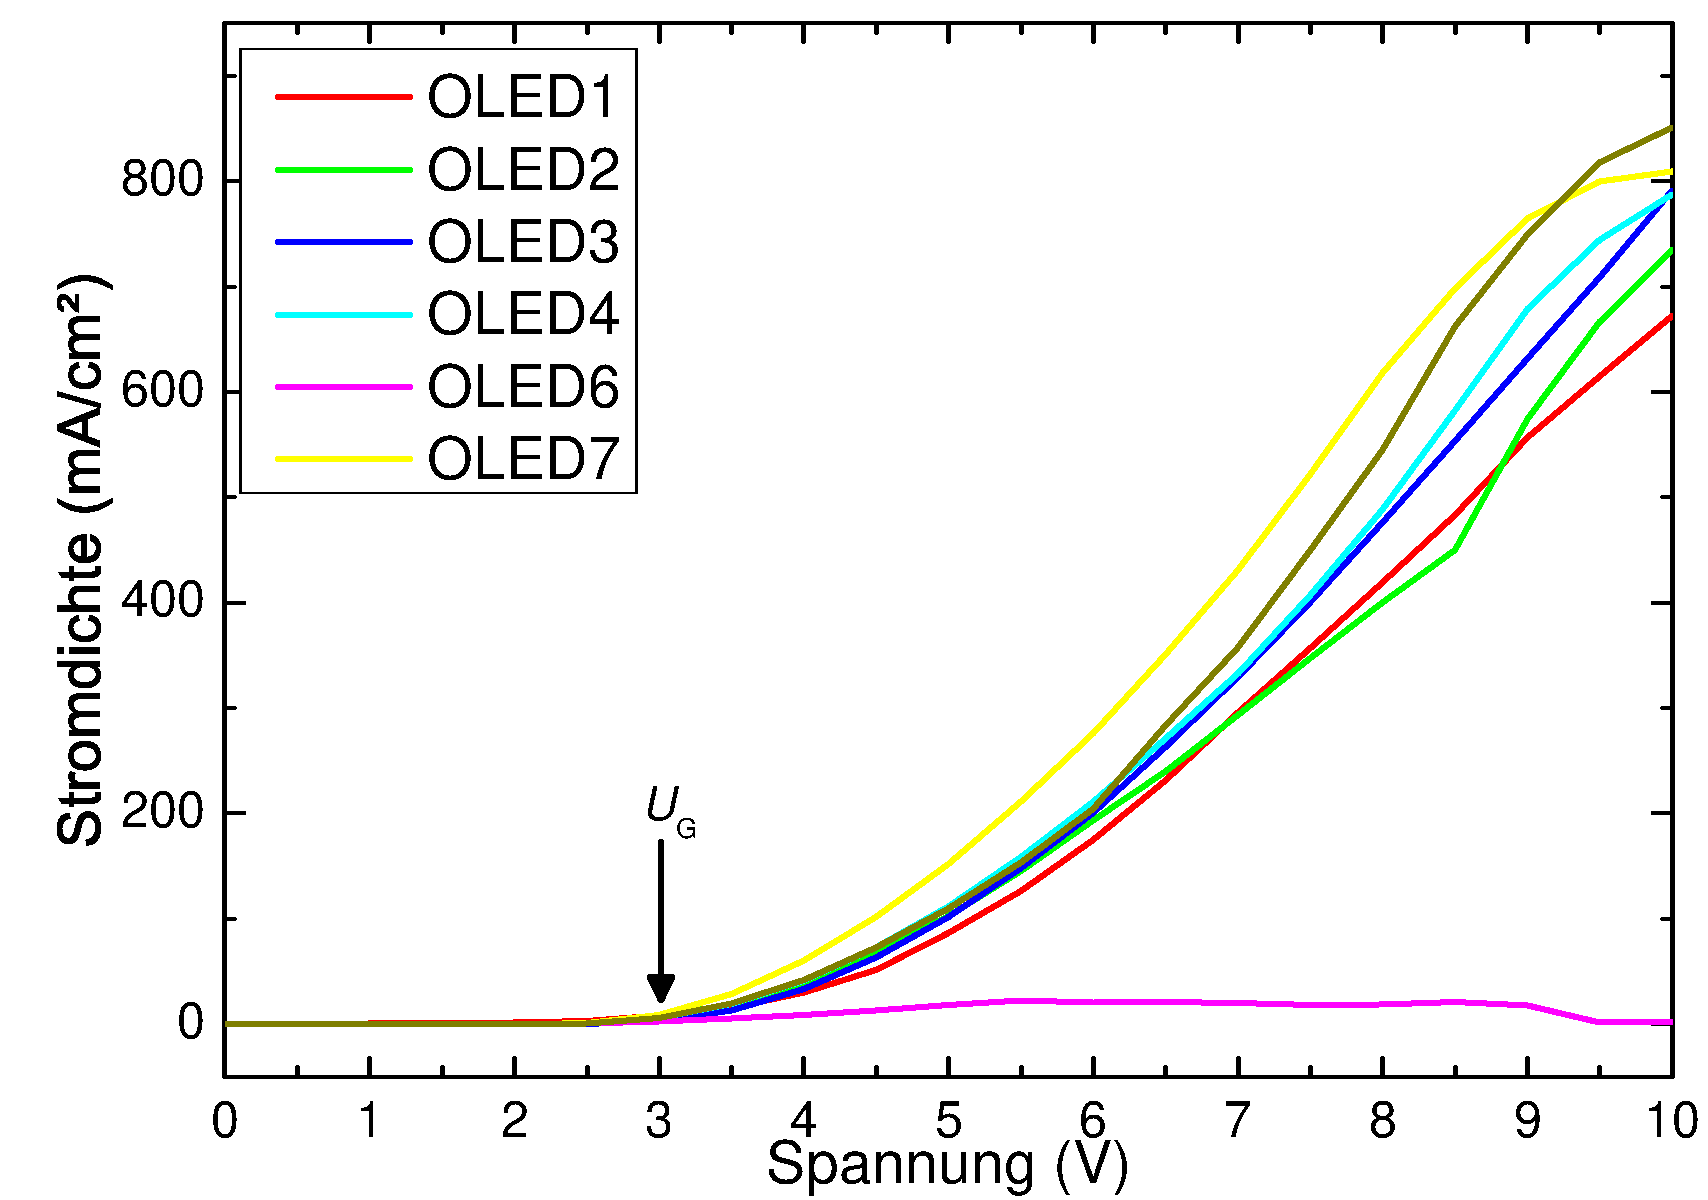
\includegraphics[width=.6\columnwidth]{Grafiken/jU-Kennlinie.pdf}%
\caption{j/U-Kennlinien aller hergestellter Proben. Ab einer Grenzspannung $U_{\mathrm{G}}$ nimmt der Strom exponentiell mit der Spannung zu wachsen. Gegen 10~V ist das Eintreten einer S�ttigung zu erkennen. Die Stromdichte von OLED6 w�chst zu beginn auch exponentiell an, ist aber ungef�hr eine Gr��enordnung kleiner als die der anderen Proben.}%
\label{fig:jU-Kennlinie}%
\end{figure}

 
 
 
 




\section{Spannungsabh�ngigkeit des Spektrums}
\label{ch:Messung:sec:Spektrum}


\begin{figure}%
\centering
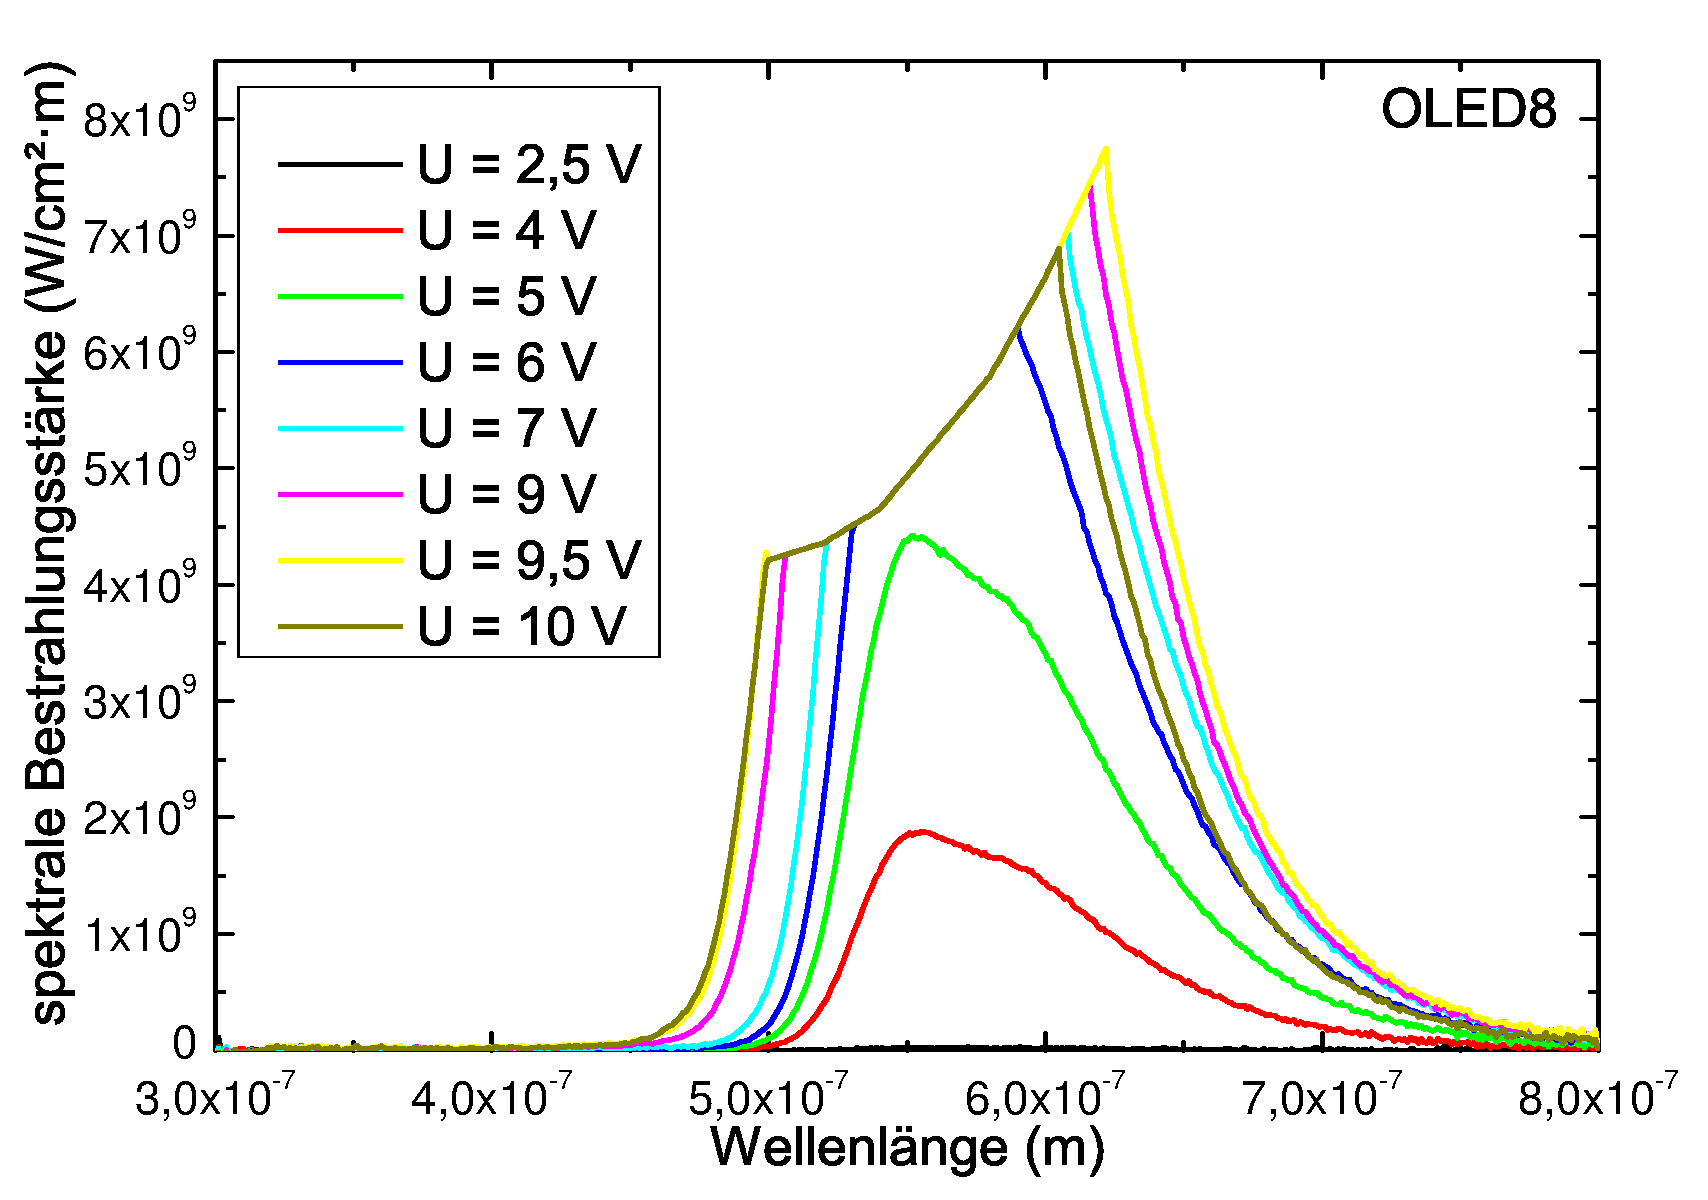
\includegraphics[width=.6\columnwidth]{Grafiken/SpektrumOLED8.pdf}%
\caption[Fehlerhafte Messungen: Aussteuerung bei hohen Spannungen]{Ab einer gewissen Spannung ist die Bestrahlung durch die OLED so gro�, dass es zu einer Aussteuerung des Messsystems kommt. Bei der gezeigten OLED8 tritt dieser Effekt ab $U$~=~6~V auf.}%
\label{fig:OLED8}%
\end{figure}

Anhand der Messdaten zeigt sich eine Spannungsabh�ngigkeit des Energiedichtespenktrums. Abbildung \ref{fig:OLED8} veranschaulicht dies. Bei einer Spannung von 2,5~V emittiert die OLED noch keine Strahlung. Mit zunehmender Spannung nimmt die maximale Bestahlungsst�rke und auch die Breite des Spektrums zu.

Auch die Leuchtdichte f�ngt ab der Grenzspannung $U_{\mathrm{G}}$ an zu steigen. Zun�chst nimmt die Leuchtdichte exponentiell mit der Spannung zu. Bei OLED1 und OLED2 zeigt sich bei hohen Spannungswerten eine Abnahme der Leuchtdichte. Hieraus folgt, dass die Leuchtdichte f�r OLED1 und OLED2 im untersuchten Bereich ein Maximum zwischen den Messwerten hat.
Aufgrund der Aussteuerung des Messystems (vgl. Abschnitt \ref{ch:Messung:sec:Fehler}) sind die gemessenen Werte der Leuchtdichte bei den �brigen OLEDs nicht verwendbar. Allerdings kann man anhand Breite und H�he der Spektren bei hohen Spannungswerten ein Abnehmen der Leuchtdichte annehmen. In Abbildung \ref{fig:OLED8} ist dies f�r den Spannungswert $U = 10$~V zu erkennen, der in H�he und Breite kleiner als das Spektrum bei 9~V ist.

Der Anstieg der Leuchtdichte mit steigender Spannung l�sst sich durch eine steigende Anzahl von Ladungstr�gern und damit eine erh�hte Wahrscheinlichkeit zur Excitonenbildung und damit zur strahlenden Rekombination. Ab einer bestimmten Spannung kann eine Abnahme der Leuchtdichte beobachtet werden. Durch hohe Felder k�nnten die Ladungstr�ger sehr schnell durch die Emissionszone beschleunigt werden und in die Elektroden gelangen. Damit verringert sich die Wahrscheinlichkeit zur strahlenden Rekombination.

Weitergehend kann aus Abbildung \ref{fig:OLED8} abgeleitet werden, dass sich das Maximum der spektralen Bestrahlungsst�rke durch eine Erh�hung der Spannung nicht ver�ndert. Dies kann dadurch erkl�rt werden, dass das Emissionsspektrum vom Abstand zwischen HOMO und LUMO abh�ngt. Dieser Abstand ist materialabh�ngig und wird daher nicht durch die Spannung beeintr�chtigt.  


%a.) Typischer diodenkennlinienverlauf
%		Kein Stromfluss bis ~3 V
%		OLED1: Ohmscher Anteil darunter
%		
%		Erkl�rung f�r Diodenkennlinie:
%		- Ab dieser spannung "`flachbandfall"' siehe Grundlagen
%		- 
%
%
%-  Ohmscher Anteil parellel zur Diode bei OLED1
%
%- Probe OLED1 und OLED2: Geringere Stromdichte als alle anderen
%	H�herer Widerstand
%	Schlechtere Ladungstr�gerinjektion in Organik
%	wegen: Fehlendes PEDOT:PSS
%		
%
%
%- 
%
%

\begin{figure}%
\centering
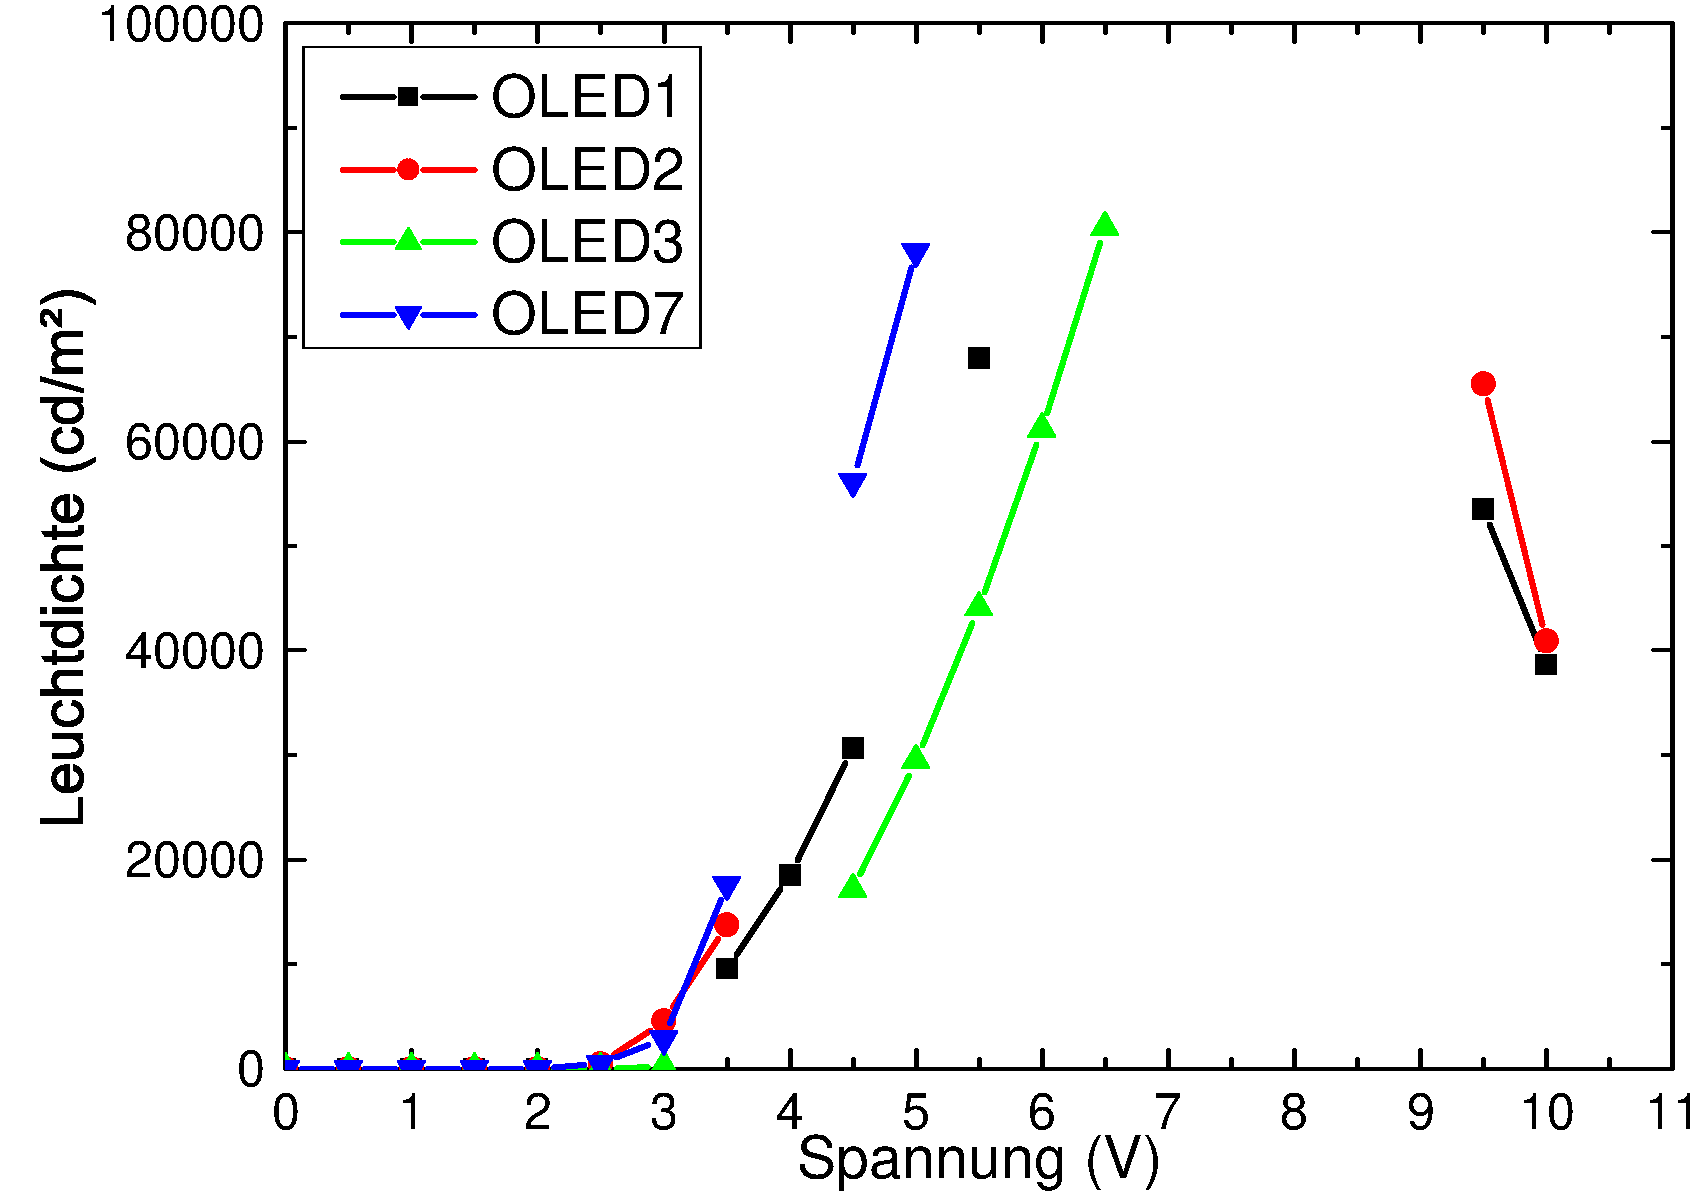
\includegraphics[width=.6\columnwidth]{Grafiken/PEDOT_Leuchtdichte.pdf}%
\caption[Leuchtdichte/Spannungsdiagramm]{Die Abbildung zeigt die Abh�ngigkeit der Leuchtdichte von der Spannung. Spannungswerte mit Messfehlern tauchen nicht im Diagramm auf. Ab einer Grenzspannung steigt die Leuchtdichte exponentiell an. Bei hohen Spannungen ist ein abfallen der Leuchtdichte zu erkennen.}%
\label{fig:PEDOT_Leuchtdichte}%
\end{figure}



%
%- Zunahme der Energiedichte f�r steigende Spannung
%	
%- Ab bestimtmer Spannung sinkt Energiedichte wieder ab
%   --> bei OLED1+2 leichte verschiebung des Maximums
%   
%   
\section{Einfluss von PEDOT:PSS}
\label{ch:Messung:sec:PEDOT}


\begin{figure}%
\centering
\begin{adjustwidth}{-1.2cm}{0cm}
	\subfloat[$U$ = 0 - 4 V]{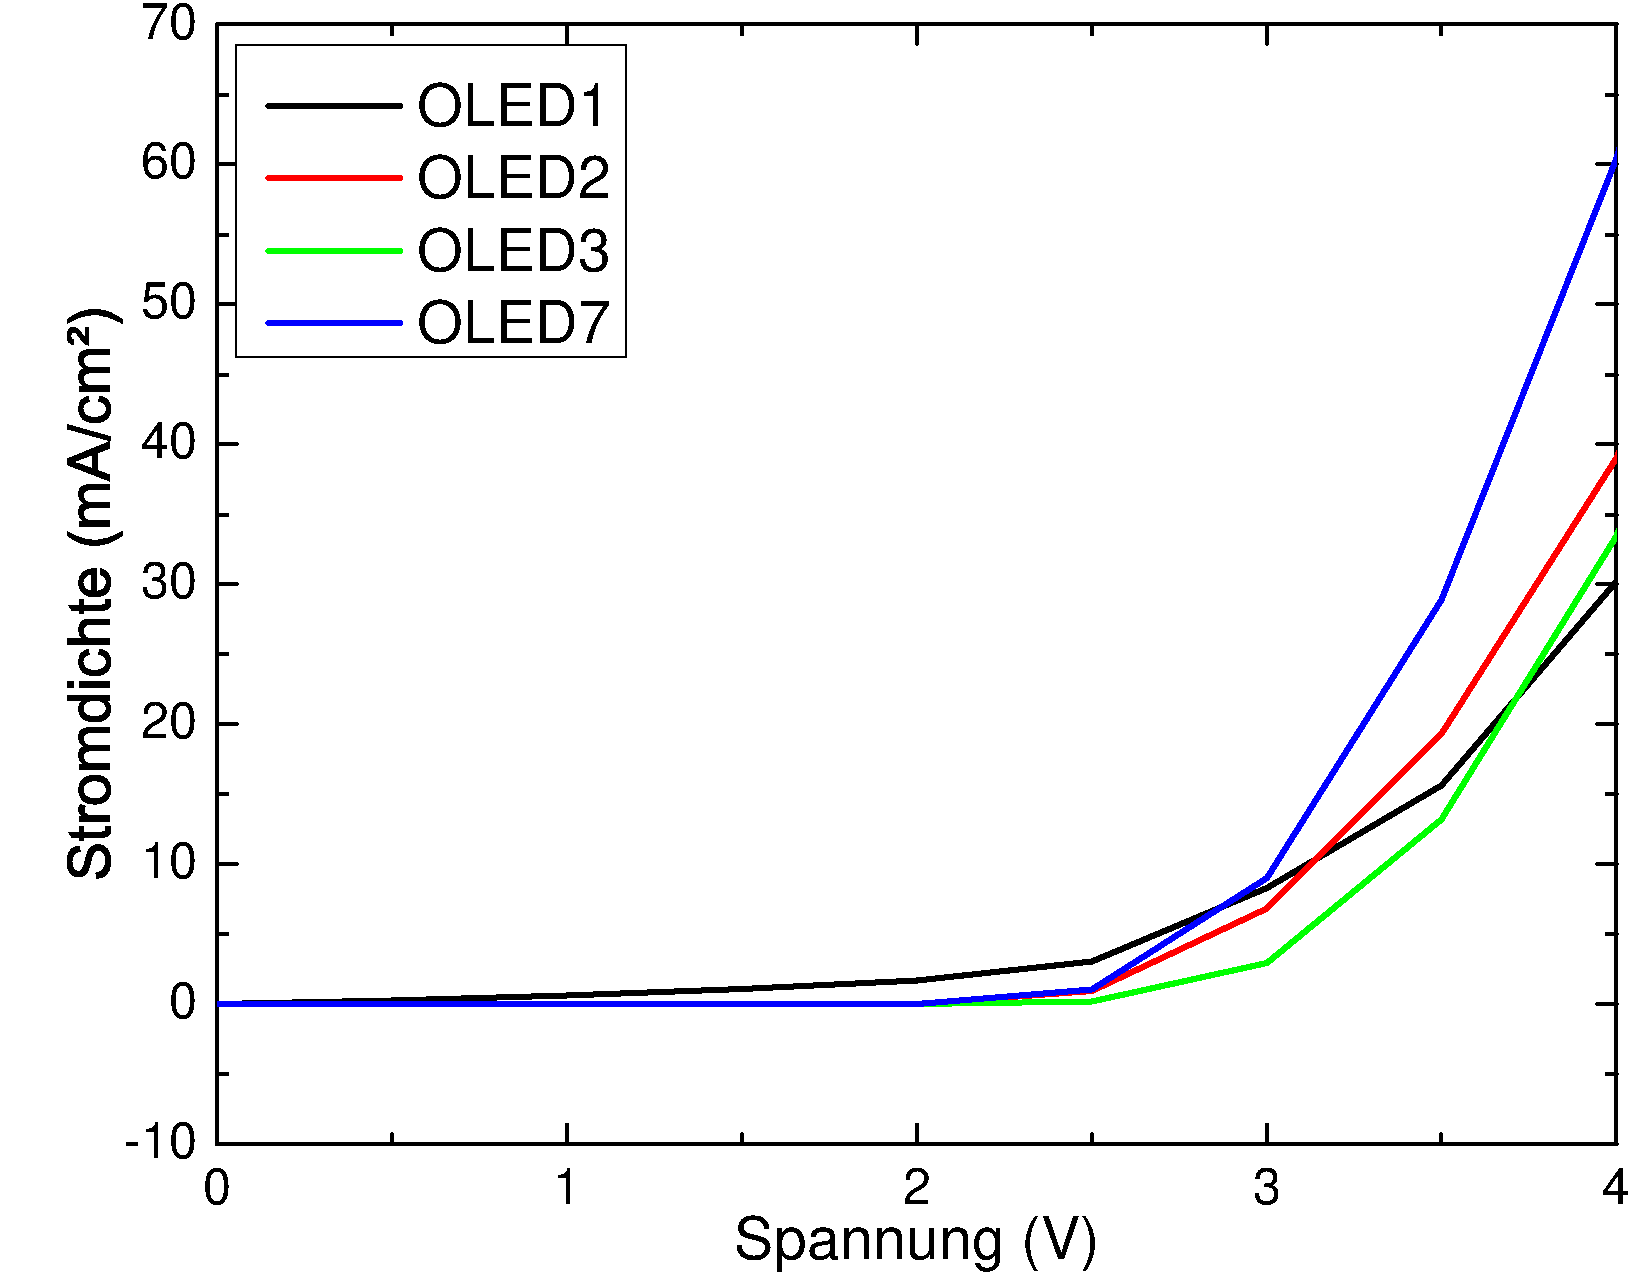
\includegraphics[width=.58\columnwidth]{Grafiken/jU_PEDOT_ausschnitt.pdf}\label{fig:jUPEDOT_ausschnitt}}
	\subfloat[$U$ = 0 - 10 V]{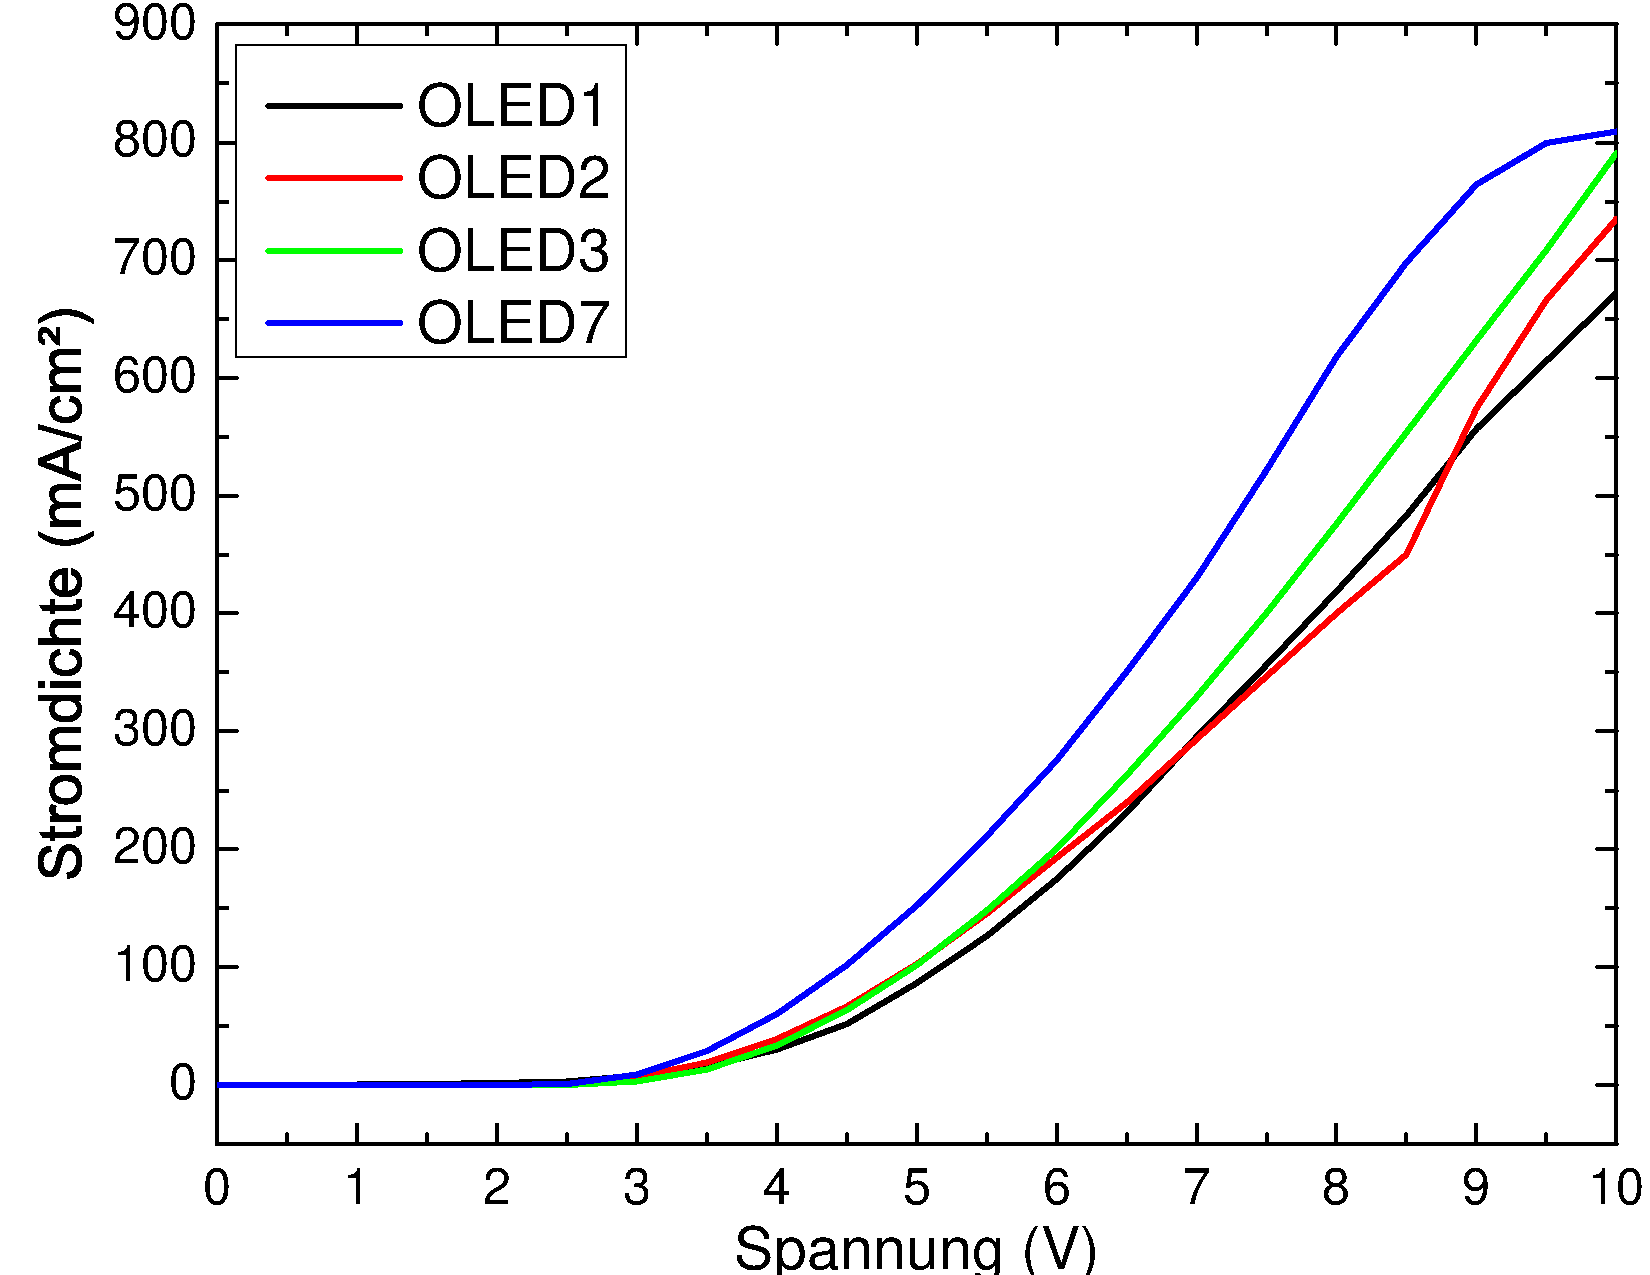
\includegraphics[width=.58\columnwidth]{Grafiken/jU_PEDOT.pdf} \label{fig:jUPEDOT}}%
	\end{adjustwidth}
\caption[j/U-Kennlinien: OLED mit und ohne PEDOT:PSS]{Auswirkung von PEDOT:PSS auf $j/U$-Kennlinien: OLED1, OLED2 ohne PEDOT:PSS, OLED3, OLED7 mit PEDOT:PSS. \textbf{(a)} Im Ausschnitt der j/U-Kennlinie kann man die Grenzspannung $U_{\mathrm{G}}$ f�r die gezeigten OLEDs erkennen. \textbf{(b)} Ab der Grenzspanspannung steigt die Stromdichte stark an, bis sie gegen Ende der Kurve abflacht.}%
\label{fig:jUPedot_sub}%
\end{figure}
Bei der Herstellung wurden Proben sowohl mit, als auch ohne PEDOT:PSS hergestellt.
Anhand Abbildung \ref{fig:jUPedot_sub} soll nun die Auswirkung dieser PEDOT:PSS Schicht als Injektionsschicht auf die hergestellten Proben untersucht werden. OLED1 und OLED2 wei�en keine PEDOT:PSS Schicht auf, OLED3 und OLED7 haben eine $\sim$18~nm dicke PEDOT:PSS Schicht. Auf alle vier Proben wurden $\sim$60~nm  "`Super Yellow"' aufgebracht (vgl. \todo{ref auf Tabelle}).
In Abbildung \ref{fig:jUPEDOT_ausschnitt} ist die Stromdichte der vier Proben �ber der Spannung im Bereich von 0~-~4~V zu erkennen. Ab 3~V sind bei allen Proben Str�me zu messen. Eine Ver�nderung der Grenzspannung $U_{\mathrm{G}}$ durch den Einsatz von PEDOT:PSS ist nicht zu beobachten. Bei der Probe OLED7 steigt die Stromdichte oberhalb von  $U_{\mathrm{G}}$ wesentlich schneller an, als bei den Proben ohne PEDOT:PSS. Da die Stromdichte von OLED3 im Spannungsbereich von 0~-~4~V aber langsamer als die anderen Proben ansteigt, kann keine Aussage �ber den Einfluss von PEDOT:PSS auf die Stromdichte in diesem Spannungsbereich gemacht werden.

Beim Betrachten von \ref{fig:jUPEDOT} zeigt sich, dass beide Proben mit PEDOT:PSS bei Spannungen $U~>~6$~V eine h�here Stromdichte aufwei�en, als die Proben ohne. Die vergleichsweise h�here Stromdichte l�sst sich auf die erleichterte Injektion von Ladungstr�gern durch die PEDOT:PSS-Schicht zur�ckf�hren.


\section{Auswirkung der Emitterschichtdicke}
\label{ch:Messung:sec:Dicke}

Bei der Herstellung wurden Proben mit unterschiedlicher Drehzahlen beim Aufbringen der Emitterschicht hergestellt.
Hieraus resultieren unterschiedliche Schichtdicken. 
Die Proben OLED3 und OLED7 haben eine Emitterschtdicke von $\sim60$~nm. OLED6 hat eine Emitterschichtdicke zwischen 30~nm und 40~nm. Die Proben OLED4 und OLED8 wurden bei geringer Drehzahl (500~min$^-1$ f�r 55~s) hergestellt. Daraus folgt eine wesentlich h�here Schichtdicke. Unter der Annahme, dass kein Material von der Probe geschleudert wird, kann eine maximale Schichtdicke abgesch�tzt werden. Mit 120 $\upmu$l "`Super Yellow"' folgt damit:

\begin{equation}
d=\frac{V}{A}=\frac{120~\upmu \mathrm{l}}{(16~\mathrm{mm})^2}=4,7~\upmu \mathrm{m}
\label{eq:dicke}
\end{equation}
Die reale Schichtdicke wird allerdings etwas geringer sein. Durch die geringe Drehzahl ist weitergehend mit einer inhomogenen Schicht zu rechnen und auch ein Androcknen des Lackes ist denkbar. 

\begin{figure}%
\centering
\begin{adjustwidth}{-1.1cm}{0cm}
	\subfloat[$U$ = 4,5~V]{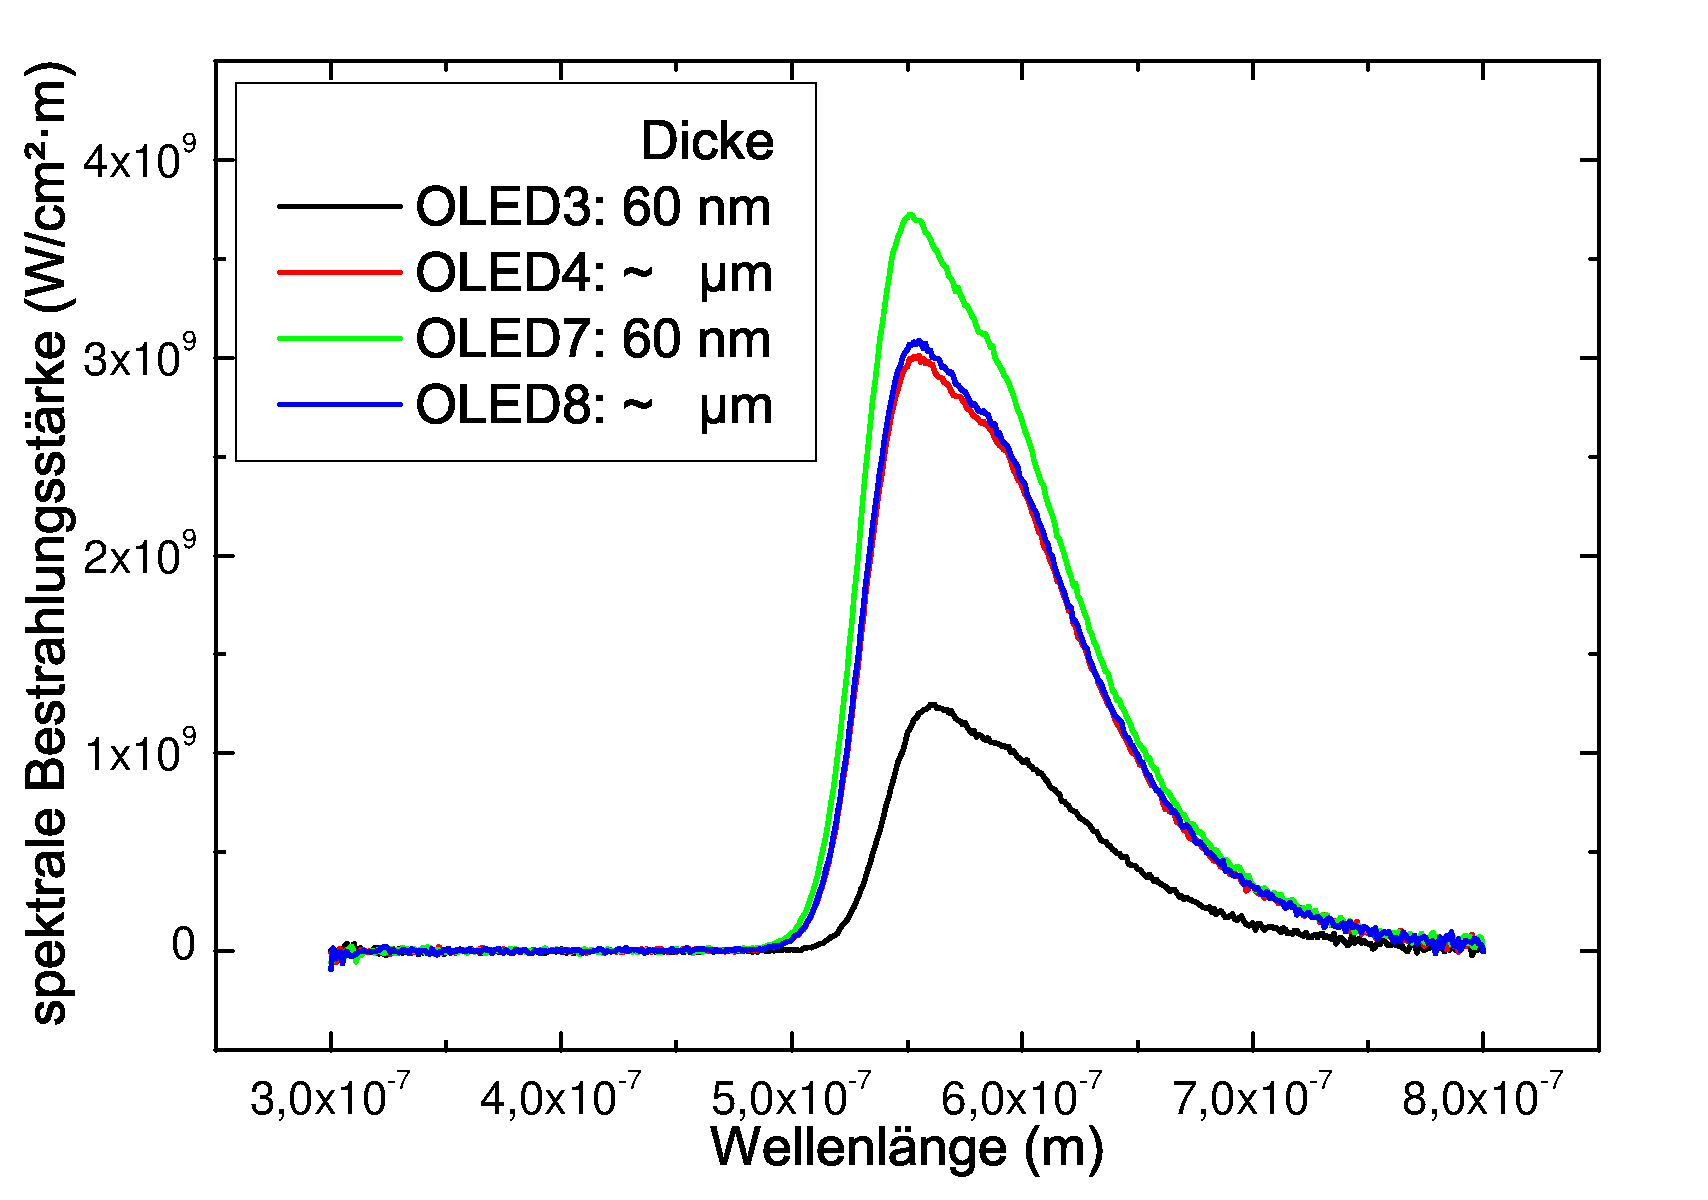
\includegraphics[width=.58\columnwidth]{Grafiken/Spektrum_45V.pdf}\label{fig:Spektrum4.5}}
	\subfloat[$U$ = 5~V]{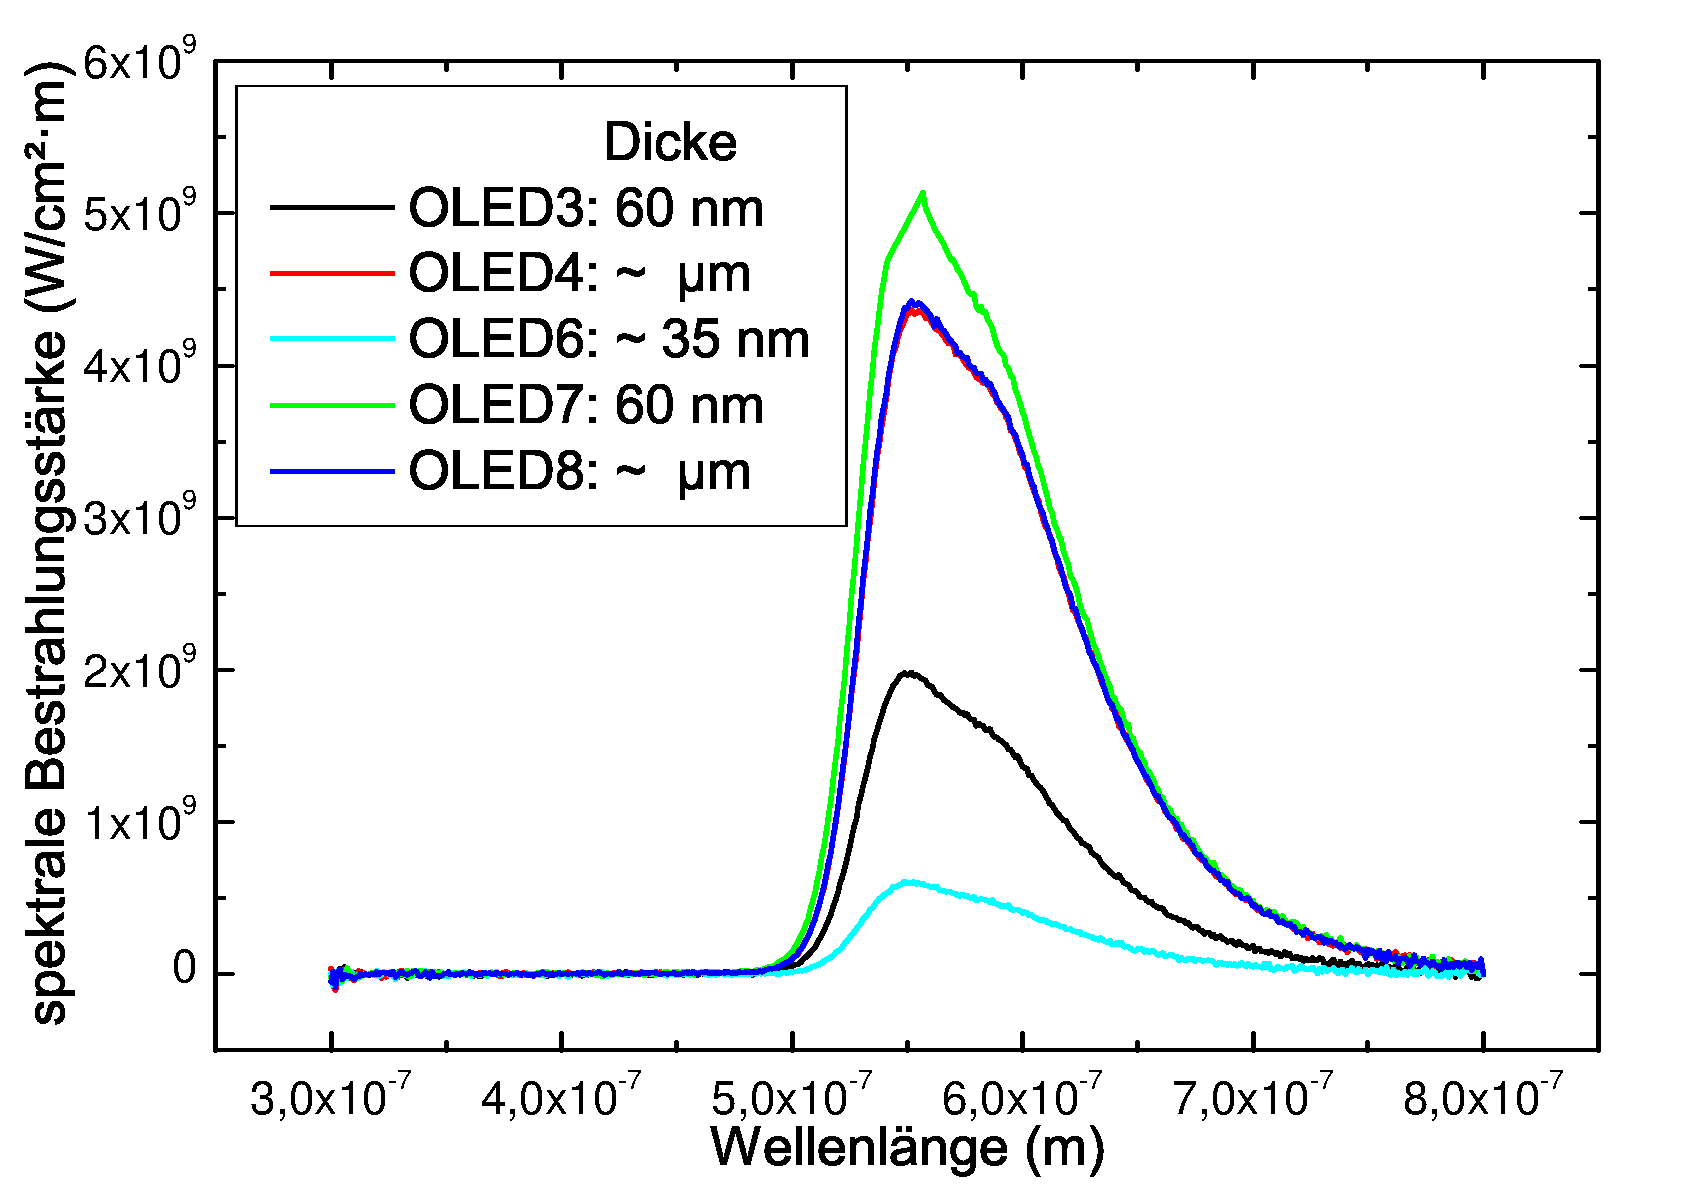
\includegraphics[width=.58\columnwidth]{Grafiken/Spektrum_5V.pdf} \label{fig:Spektrum5}}%
	\end{adjustwidth}
\caption[Spektren unter Variation der SY-Dicke]{
 Spektren der Bestrahlungsst�rke f�r unterschiedlichen Schichtdicken der Emissionsschicht. \textbf{(a)} Bei einer Spannung von 4,5~V sind keine fehlerfreie Messwerte von OLED6 vorhanden. 
 \textbf{(b)} Bei einer Spannung von 5~V kommt es zu einem Aussteuern des Messystems bei OLED7.}%
\label{fig:SpektrumSchichtdickes}%
\end{figure}



%% --------------------
%% |   Bibliography   |
%% --------------------
\cleardoublepage
\phantomsection
\addcontentsline{toc}{chapter}{\bibname}

\iflanguage{english}
{\bibliographystyle{IEEEtranSA}}	% english style
{\bibliographystyle{babalpha-fl}}	% german style
												  
% Use IEEEtran for numeric references
%\bibliographystyle{IEEEtranSA})

\bibliography{thesis}
\nocite{*}


%% ----------------
%% |   Appendix   |
%% ----------------
\cleardoublepage

%% appendix.tex
%%

%% ==============================
%\chapter{Appendix}
%\label{ch:Appendix}
%% ==============================

\appendix

\iflanguage{english}
{\addchap{Appendix}}	% english style
{\addchap{Anhang}}	% german style


\section{First Appendix Section}
		\label{Anhang-Implementierung}
		
\setcounter{figure}{0}
		
\begin{figure} [ht]
  \centering
   ein Bild
  \caption{A figure}
  \label{fig:BPMNBeispiela}
\end{figure}


\dots






\end{document}
